%% ============================================================
%%  Variogram-based GPR on industrial copper-molybdenum flotation data
%%  Draft -- arXiv preprint
%% ============================================================
\documentclass[final,11pt,nopreprintline]{elsarticle}

\usepackage{amsmath}
\usepackage{amssymb}
\usepackage{graphicx}
\graphicspath{{../figures/}{figures/}}
\usepackage{hyperref}
\hypersetup{colorlinks=true,linkcolor=black,citecolor=black,urlcolor=black,filecolor=black,pdfhighlight=/N}
\AtBeginDocument{\hypersetup{linkcolor=black,citecolor=black,urlcolor=black,filecolor=black}}
\usepackage{microtype}
\usepackage{booktabs}

\renewcommand{\topfraction}{0.92}
\renewcommand{\bottomfraction}{0.75}
\renewcommand{\textfraction}{0.06}
\renewcommand{\floatpagefraction}{0.85}
\setcounter{topnumber}{2}
\setcounter{totalnumber}{4}
\setlength{\textfloatsep}{12pt plus 2pt minus 2pt}
\setlength{\intextsep}{12pt plus 2pt minus 2pt}

\journal{Minerals Engineering}

\begin{document}
\begin{frontmatter}

\title{Applicability of variogram-based Gaussian process regression to
industrial flotation data: a copper--molybdenum case study}

\author{Sicheng Mu\corref{cor1}}
\ead{sichengmu2026@163.com}
\affiliation{organization={School of Resources Engineering},
  addressline={Xi'an University of Architecture and Technology},
  city={Xi'an}, postcode={710055}, state={Shaanxi}, country={China}}
\cortext[cor1]{Corresponding author.}

\begin{abstract}
Variogram-based Gaussian process regression has recently been
demonstrated as a probabilistic framework for optimising mineral
processing circuits, with validation on a statistically designed
flotation campaign. Its applicability to plant campaign data, which are
typically acquired one factor at a time and are subject to measurement
noise, has not been examined. The present study applies the published
workflow, without modification, to thirty-eight flotation tests from a
copper--molybdenum concentrator. Predicted recoveries outside the
physically admissible range are obtained over a substantial fraction of
the interpolated domain, and the reported Pareto frontier is not
reproducible under posterior resampling. Three modelling assumptions
account for these observations, and modifications to each are proposed
and evaluated by leave-one-out cross-validation. The modified workflow
yields predictions that satisfy physical bounds, an uncertainty estimate
consistent with the observed measurement variability, and an operating
window that agrees with independent conclusions drawn from the same
campaign.
\end{abstract}

\begin{keyword}
froth flotation \sep Gaussian process regression \sep uncertainty
quantification \sep multi-objective optimisation \sep
copper--molybdenum separation
\end{keyword}
\end{frontmatter}

\section{Introduction}

The progressive depletion of high-grade, readily processed sulphide ores
has increased the sensitivity of flotation performance to variations in
feed mineralogy and pulp chemistry, narrowing the range of operating
conditions over which target grades and recoveries can be maintained
simultaneously. Copper--molybdenum separation illustrates the difficulty
well, since molybdenite and chalcopyrite are both naturally hydrophobic
and the reagent regimes that promote the flotation of one generally
promote the flotation of the other as well.

Surrogate models that predict metallurgical response from operating
variables, and that quantify the confidence associated with each
prediction, are consequently of practical value. Gaussian process
regression is well suited to this setting: it performs comparatively well
on small datasets and provides a posterior variance as an intrinsic part
of its output rather than as a separate estimate.

The specification of the prior covariance function is a central question
in such applications. Eskanlou, Yin and Caers proposed deriving it
directly from the data through empirical variograms fitted in the space
of the operating variables, and demonstrated the approach on a designed
flotation campaign, reporting a Pareto-efficient frontier between two
competing responses which could be mapped back to process settings. The
formulation is attractive because the covariance structure is estimated
rather than assumed, and the accompanying implementation has been made
openly available.

The present work examines how this framework behaves when it is applied
to data of a different character. Designed experiments distribute
observations through the predictor space and are conducted under
controlled conditions; plant campaign data are acquired one factor at a
time, populate the space along coordinate directions, and carry
measurement variability that a designed programme is intended to
minimise. Whether the framework transfers between these two regimes is a
question of practical consequence for industrial application, and it is
the question addressed here.

\section{Data}

The dataset originates from a molybdenum concentrator at Jinduicheng,
Shaanxi Province, China, where chalcopyrite occurs as a penalty impurity
in the molybdenite concentrate. Seasonal variation in the copper content
of the concentrate motivated a two-year experimental campaign, in which
grinding fineness, pulp pH, diesel collector dosage and diesel--pulp
conditioning time were varied while molybdenum and copper recovery were
measured on the rougher concentrate. Thirty-eight tests were available
for analysis; the ranges of the variables and responses are summarised in
Table~\ref{tab:data}.

\begin{table}[htbp]
\centering
\caption{Operating variables and metallurgical responses measured on the
rougher concentrate.}
\label{tab:data}
\begin{tabular}{llll}
\toprule
 & Variable & Range & Unit \\
\midrule
$x_1$ & Grinding fineness ($-0.074$~mm) & 40--75 & \% \\
$x_2$ & Pulp pH & 3.5--11 & -- \\
$x_3$ & Diesel dosage & 50--200 & g/t \\
$x_4$ & Conditioning time & 5--25 & min \\
\midrule
$y_1$ & Mo recovery & 7--58 & \% \\
$y_2$ & Cu recovery & 2--52 & \% \\
\bottomrule
\end{tabular}
\end{table}

Two characteristics of the data acquisition are relevant to the analysis
that follows. The campaign was conducted in a one-factor-at-a-time
manner, which is the usual practice for plant trials, with the
consequence that the thirty-eight observations are distributed along a
limited number of coordinate directions rather than throughout the
interior of the four-dimensional predictor space. In addition, pulp pH
was varied in only one of the test series, so that for the greater part
of the dataset this variable remains constant.

\section{Behaviour of the reference workflow}

The published procedure comprises the following steps: the predictors are
scaled to the unit interval; the standardised responses are reduced to
two principal components; an empirical variogram is fitted to each
component as a function of the predictor coordinates; ordinary kriging is
performed; an ensemble of conditional realisations is generated on an
augmented grid; each realisation is transformed back through the inverse
principal component and standardisation steps; and the Pareto frontier of
the ensemble mean surface is computed.

Three elements of this sequence are adopted in the original work without
accompanying sensitivity analysis, and each is examined below with
respect to the present dataset.

The first concerns the treatment of the principal components.
Independently simulated realisations of $\mathrm{PC}_1$ and
$\mathrm{PC}_2$ are combined through the inverse principal component
transformation. Since PCA ensures that the components are uncorrelated
but not that they are independent, and since conditional simulation is a
nonlinear operation, this combination is not generally
correlation-preserving. For the present dataset, the resulting responses
lie considerably outside the convex hull of the observations; together
with an interpolation grid that extends beyond the data bounds in every
scaled coordinate, this produces the predictions shown in
Fig.~\ref{fig:failure}.

\begin{figure}[htbp]
\centering
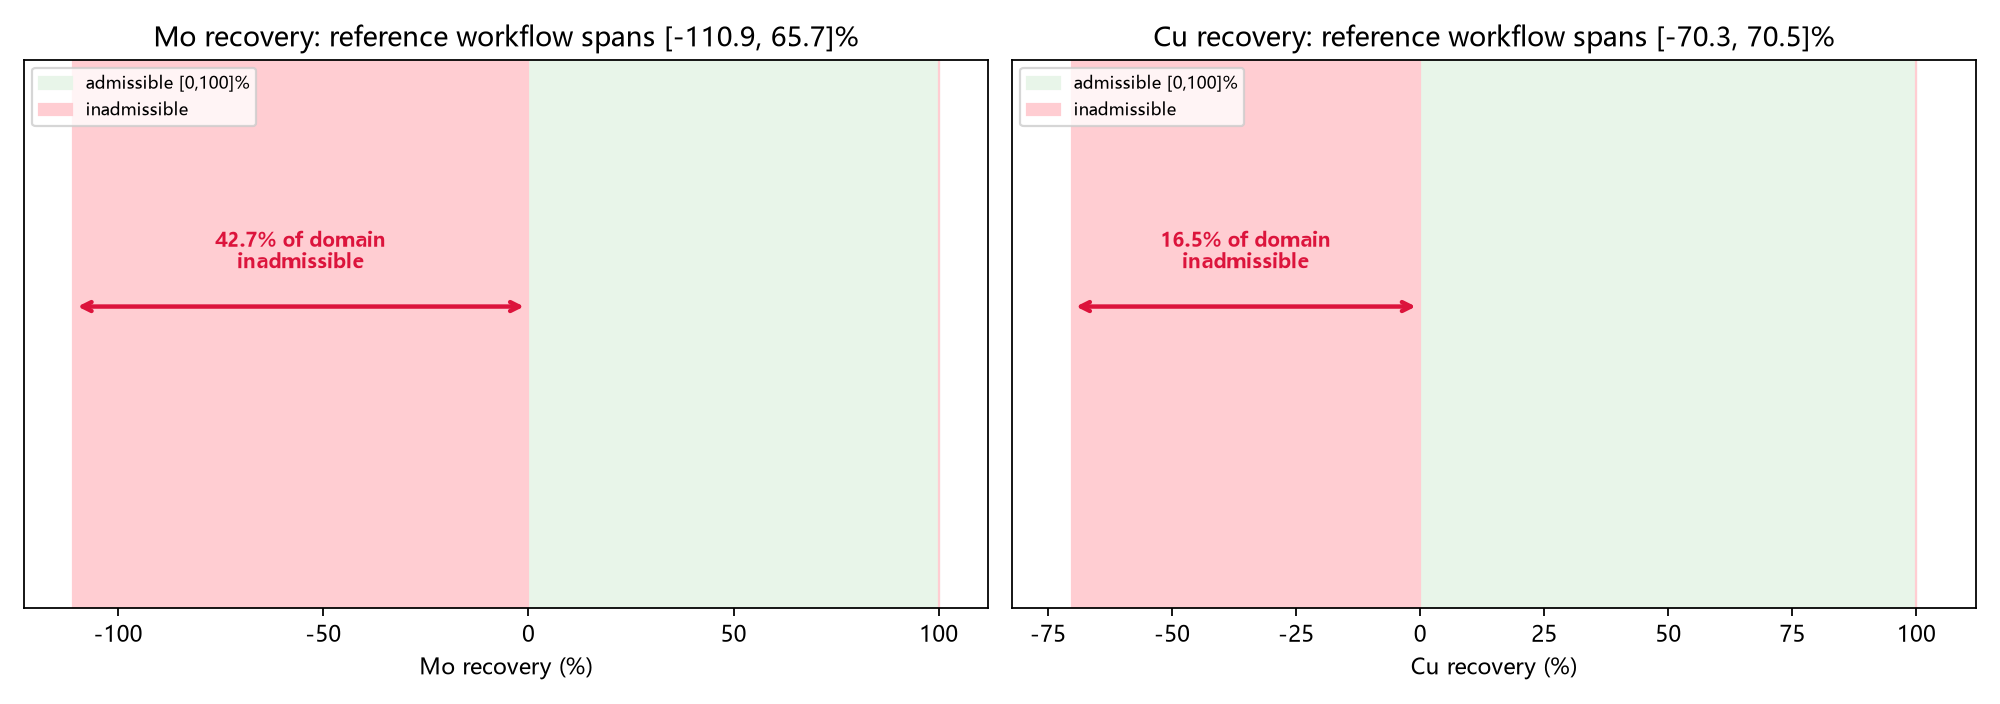
\includegraphics[width=0.95\textwidth]{Fig_failure.png}
\caption{Application of the reference workflow to the industrial
dataset. The shaded region indicates the range physically accessible to a
recovery value; the predictions obtained for molybdenum and copper
recovery fall outside this range over 42.7\% and 16.5\% of the
interpolated domain, reaching $-110.9\%$ and $-70.3\%$ respectively.}
\label{fig:failure}
\end{figure}

The second concerns the covariance structure. A single length scale is
applied to all four predictors, which implies that each influences the
response equally per unit of scaled distance. This equality refers to the
numerical scaling of the variables rather than to their relative
metallurgical significance, and it is the contrast between the two that
the subsequent analysis shows to be of interest.

The third concerns interpolation. Kriging is performed such that the
surface reproduces the observations exactly, which is appropriate for a
deterministic simulator and is not appropriate where measurement
variability is present. When the noise level is estimated from the data
rather than constrained to zero, values of $0.64$ and $0.46$ in
standardised units are obtained for the two responses, corresponding to
approximately half the response standard deviation. The reference
workflow reports zero posterior variance at these same measurement
locations. It may further be noted that the original procedure reports no
cross-validation or held-out error, so that discrepancies of this kind
are not detectable from its outputs alone.

\section{Modifications and their effect}

Four changes were made. The first three address the assumptions
identified above, and the fourth concerns the decision problem itself.

The responses were modelled directly rather than through principal
components, which removes the inverse transformation from the prediction
pathway. One process was fitted per response; this does not retain the
correlation between responses, and a co-regionalised formulation that
would do so is identified below as the natural extension, but the
predictions become physically admissible as a result.

\begin{figure}[htbp]
\centering
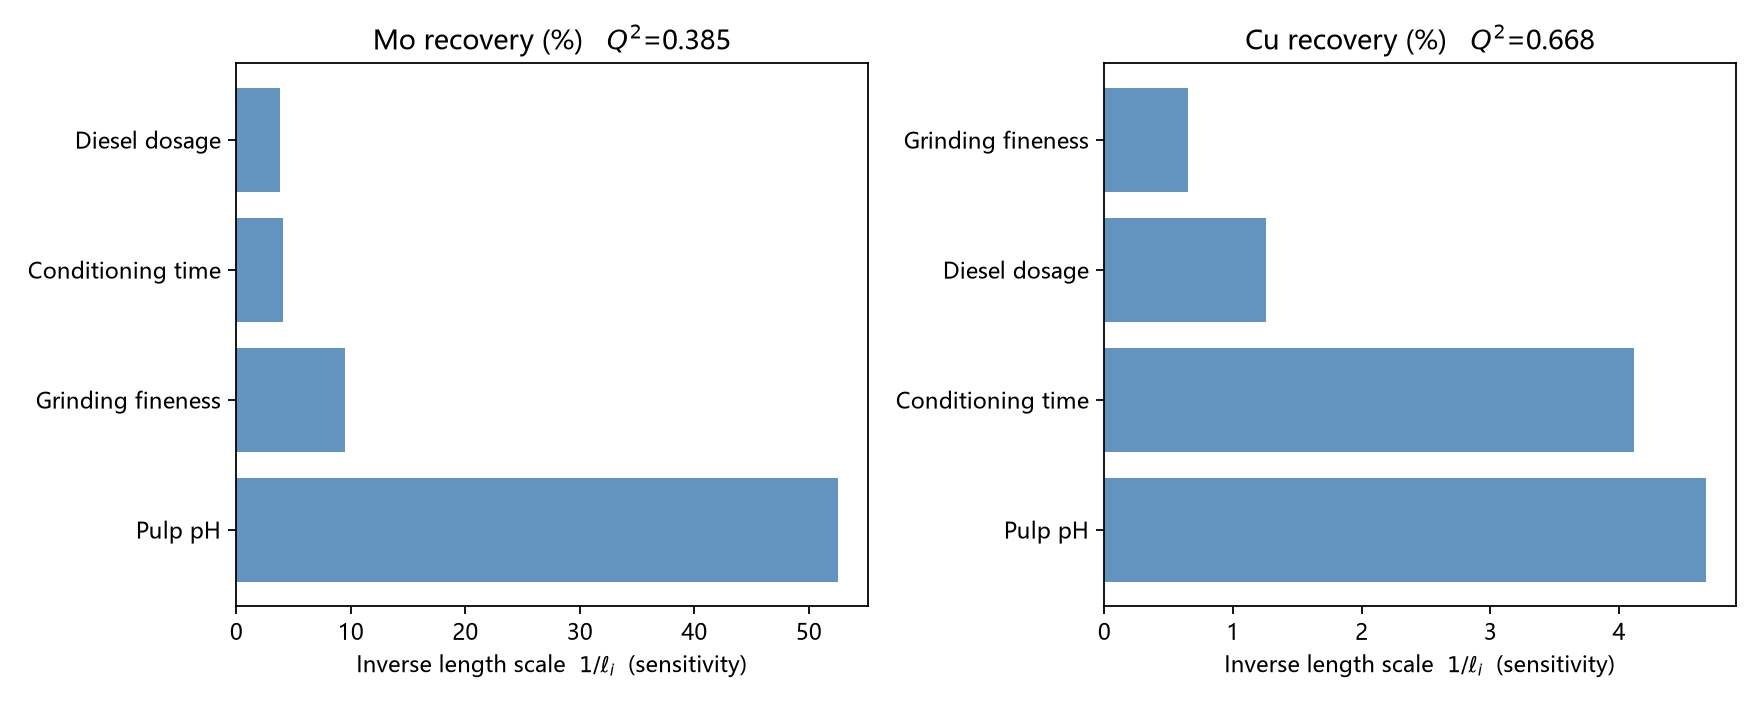
\includegraphics[width=0.92\textwidth]{Fig_ard.png}
\caption{Inverse length scales, interpreted as predictor sensitivities,
for each response. The two profiles differ both in magnitude and in
ordering.}
\label{fig:ard}
\end{figure}

An automatic relevance determination covariance function was adopted,
\begin{equation}
k(\mathbf{x},\mathbf{x}') = \sigma_f^2 \exp\!\left(
-\tfrac{1}{2}\sum_{i=1}^{d}\frac{(x_i-x_i')^2}{\ell_i^2}\right)
+ \sigma_n^2\delta_{xx'},
\end{equation}
with all hyperparameters determined by maximising the marginal
likelihood. The inverse length scales are then interpretable as
sensitivities, and are shown in Fig.~\ref{fig:ard}. Molybdenum recovery
is dominated by pulp pH, which is five and a half times more influential
than the next variable and thirteen times more influential than grinding
fineness, whereas copper recovery exhibits a flatter profile ordered
differently, with pH and conditioning time of comparable importance. A
covariance function with a single length scale cannot represent either
of these structures.

Kriging was performed in non-exact form with the nugget estimated from
the data, which allows the model to represent the finite reproducibility
of flotation testing and permits the predictive performance to be
quantified. Leave-one-out cross-validation yields coefficients of
determination of $0.39$ and $0.67$ for molybdenum and copper recovery,
with corresponding RMSE values of $10.6$ and $5.9$ percentage points
(Fig.~\ref{fig:valid}). The difference between the two is of interest:
molybdenum recovery evidently depends on variables not represented among
the four predictors, while copper recovery is more nearly determined by
them.

\begin{figure}[htbp]
\centering
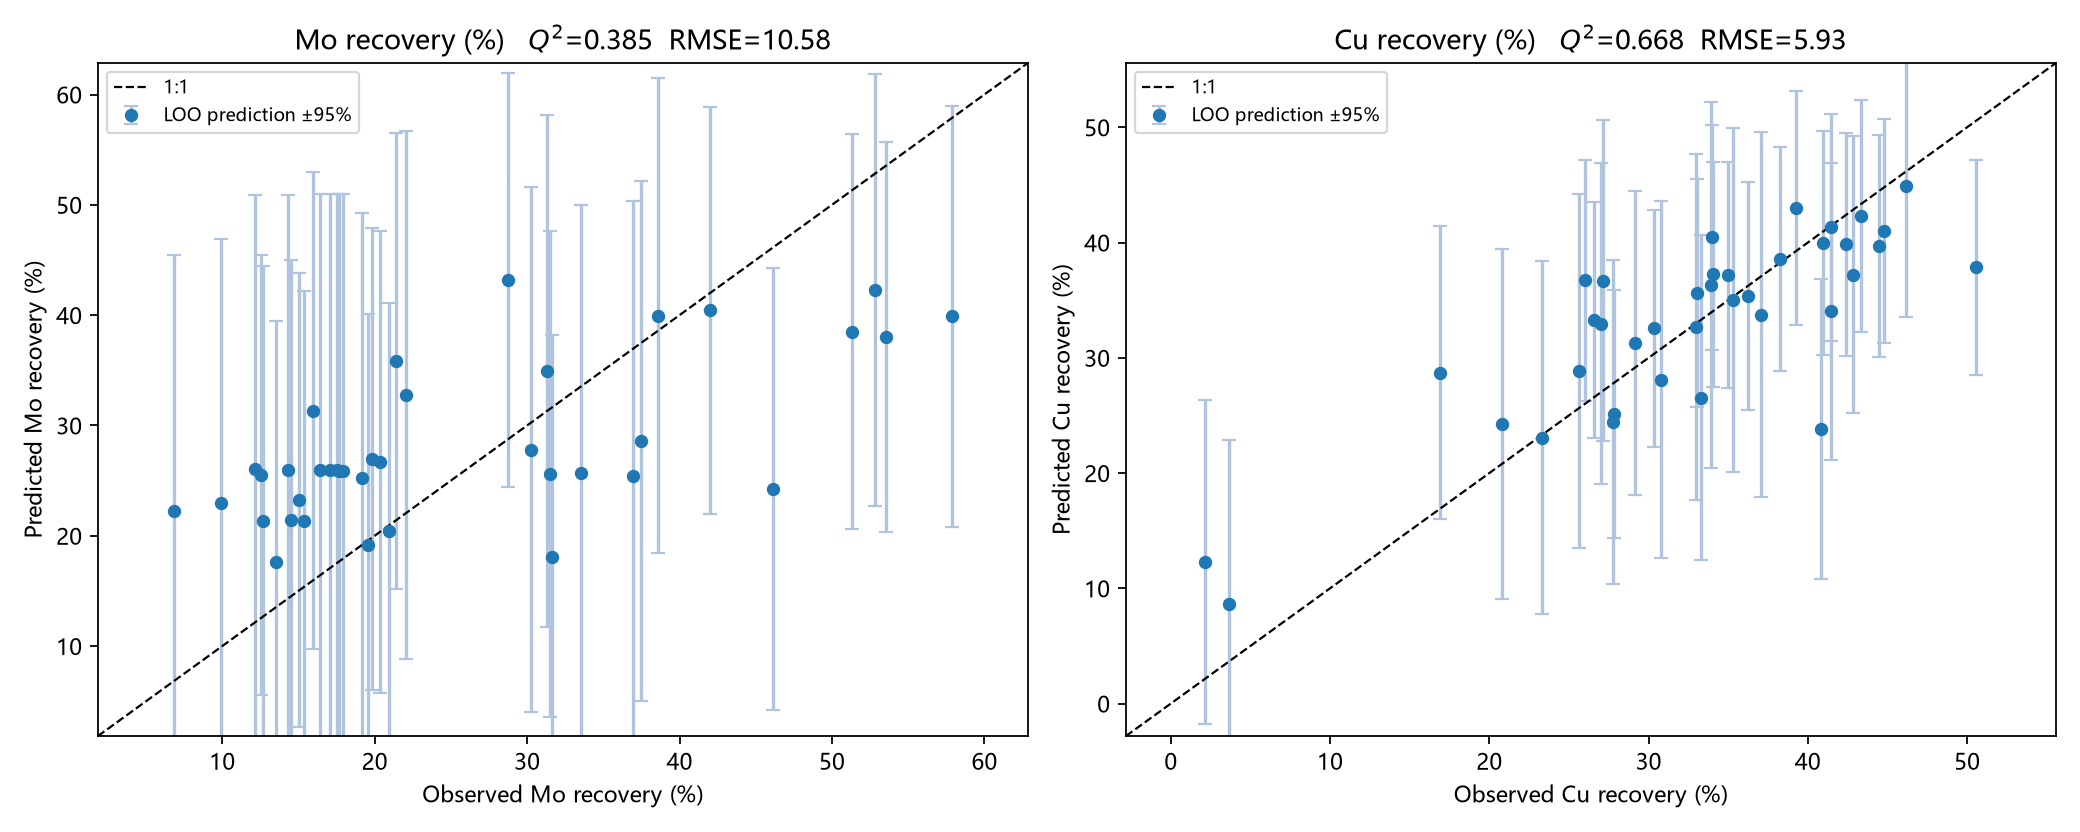
\includegraphics[width=0.95\textwidth]{Fig_validation.png}
\caption{Leave-one-out predictions against observed values, with 95\%
credible intervals.}
\label{fig:valid}
\end{figure}

The fourth modification concerns the objective formulation. Principal
component loadings of $[0.707,\,0.707]$ indicate that the two recoveries
are positively correlated over the tested conditions, so that the
efficient frontier between them is short and describes limited
trade-off. To assess the stability of the frontier, four hundred
realisations were sampled from the posterior and the frontier recomputed
for each. The mean-field frontier contains five points, and across the
four hundred realisations no point remains on the frontier in more than
ten percent of them. A chance-constrained dominance criterion was also
examined, and returned an empty set at all confidence levels tested.
These observations indicate that the Pareto formulation is not
well-posed for the present response pair.

\begin{figure}[htbp]
\centering
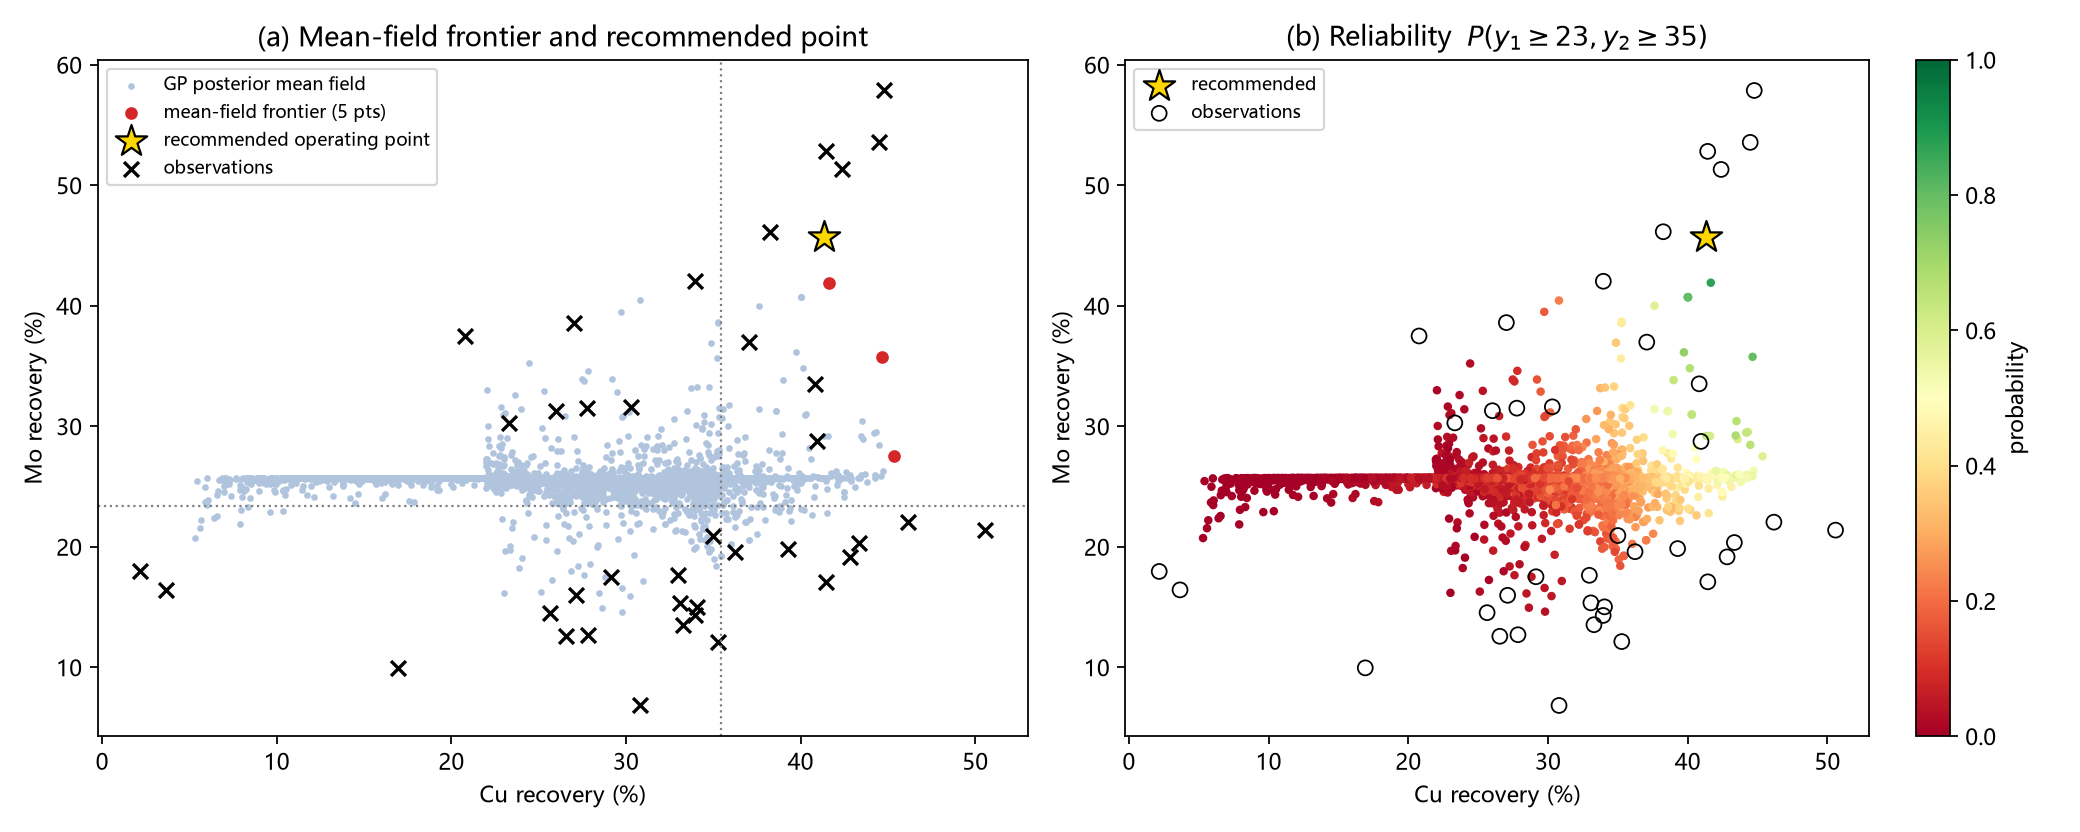
\includegraphics[width=0.95\textwidth]{Fig_frontier.png}
\caption{(a) Posterior mean field with the mean-field frontier and the
recommended operating point. (b) Probability of simultaneously exceeding
both recovery targets.}
\label{fig:frontier}
\end{figure}

An alternative formulation was therefore adopted, in which the operating
conditions are sought for which the probability of exceeding specified
recovery targets simultaneously is acceptably high. Taking the targets at
the sixtieth percentile of the observations, corresponding to
$23\%$ molybdenum and $35\%$ copper recovery, the feasible set comprises
forty-four grid points at fifty percent confidence and eight at
seventy-five percent. At ninety percent confidence the set is empty,
which indicates that the target combination is demanding given the
variability of the circuit, rather than that the analysis has failed. The
most favourable point corresponds to a grinding fineness of approximately
$70\%$, pulp pH of $7.0$, diesel dosage of $100$~g/t and conditioning
time of $15$~min, with predicted recoveries of $45.7\pm9.9\%$ for
molybdenum and $41.3\pm5.0\%$ for copper at a joint confidence of $0.88$.
The conditioning time and collector dosage obtained are consistent with
the conclusions of the original campaign, which the reference workflow
was not in a position to verify.

\section{Discussion}

The observations reported here are not specific to flotation.
Variogram-based methods were developed for spatial data, in which the
distance between two samples is a physical quantity and the variogram
summarises the spatial continuity of the phenomenon. When the same
formalism is applied in a parameter space, distance becomes a modelling
choice rather than a physical one. For a designed experiment, in which
observations are distributed through the space, the consequences of that
choice are limited. For one-factor-at-a-time plant data, the observations
lie along coordinate directions, inter-point distances are dominated by
whichever variable was varied, and an isotropic covariance function
attributes this geometrical property to physical similarity.

Several diagnostics follow, none of which require prior knowledge of the
correct result. The number of observations per effective dimension can be
counted, the extent of the interpolation grid relative to the data can be
inspected, it can be verified that predictions respect bounds known to
apply to the quantity of interest, and the stability of derived
quantities under posterior resampling can be assessed. For the present
dataset, three of these four would have identified the issues described
above before they appeared in any figure.

Two limitations should be noted. The dataset comprises thirty-eight
observations from a single deposit, and the behaviour described is
demonstrated on one case rather than established statistically; the
accompanying code permits the same diagnostics to be applied to other
datasets. In addition, modelling the responses independently forgoes the
correlation between them, which the data contain. A co-regionalised
formulation would retain this information and is considered the most
valuable immediate extension, particularly in view of the fact that the
operational decision at this concentrator concerns concentrate grade
rather than recovery, where the two objectives are in genuine conflict
and a frontier formulation would be well posed.

\section{Conclusions}

A variogram-based Gaussian process workflow that performs satisfactorily
on a designed flotation experiment does not transfer without modification
to plant campaign data. Three assumptions underlie this difference, and
each is identifiable from the data in advance: independent simulation of
principal components which are subsequently combined through a nonlinear
inverse transformation, a single correlation length applied across
predictors of unequal influence, and exact interpolation of observations
subject to measurement variability. Modifying each of these, and
replacing the Pareto frontier with a reliability-based criterion once the
responses were found not to be in conflict, produces predictions that
satisfy physical bounds, an uncertainty estimate consistent with the
observed variability, and an operating window in agreement with the
independent conclusions of the campaign. These modifications are
recommended as prerequisites for the application of variogram-based
Gaussian process regression to industrial flotation data.

\end{document}
